\documentclass[10pt]{article}
\usepackage{amsmath}
\usepackage{paralist}
\usepackage{setspace}
\usepackage{listings}
\usepackage{graphicx}
\usepackage[english]{babel}
\usepackage{geometry}
\usepackage{subcaption}
\usepackage[utf8]{inputenc}
\usepackage{listings}

\renewcommand{\figurename}{Abb.}
\renewcommand{\contentsname}{Inhaltsverzeichnis}

\begin{document}
\lstset{
	language=C,
	basicstyle=\footnotesize,
	frame=tb,
	xleftmargin=.2\textwidth,
	xrightmargin=.2\textwidth
}
\onehalfspacing
\begin{titlepage}
\begin{center}
% Oberer Teil der Titelseite:


\textsc{\LARGE Universität Oldenburg}\\[1.5cm]

\textsc{\Large Fortgeschrittene Computerorientierte Physik}\\[0.5cm]


% Title
\newcommand{\HRule}{\rule{\linewidth}{0.5mm}}
\HRule \\[0.4cm]
{ \huge \bfseries Verteilung der kürzesten Pfade in skalenfreien Graphen}\\[0.4cm]

\HRule \\[1.5cm]

% Author and supervisor
\begin{minipage}{0.4\textwidth}
\begin{flushleft} \large
\emph{Author:}\\
Jan \textsc{K\"amper}\\
Florian \textsc{B\"orgel}
\end{flushleft}
\end{minipage}
\hfill
\begin{minipage}{0.4\textwidth}
\begin{flushright} \large
\emph{Supervisor:} \\
Alexander \textsc{Hartmann}
\end{flushright}
\end{minipage}
\\[3cm]
\vfill



% Unterer Teil der Seite
{\large \today}

\end{center}

\end{titlepage}
\tableofcontents
\newpage
\section{Problemstellung}
 
Ziel dieses Projektes ist es, statistische Beobachtungen über die Verteilung von kürzesten Pfaden in skalenfreien Graphen sowie in ebenen Zufallsgraphen zu machen. In skalenfreien Graphen sind die Kanten pro Knoten nach einem Potenzgesetz verteilt: 
\begin{equation*}
P(k) \sim k^{-\alpha}
\end{equation*}
Die Erstellung von skalenfreien Graphen erfolgt durch spezielle Algorithmen. Der hier verwendete Algorithmus basiert auf dem Barabasi-Albert Model (siehe \cite{Barabasi}) und nutzt die Methode Preferential Attachment. Dabei ist der Parameter $m$ maßgeblich, der die Anzahl an Nachbarn eines neu hinzugefügten Knotens beschreibt. \\

Die Größe des Graphen wird über die Anzahl der Knoten $n$ definiert. Um eine Aussage über die statistische Verteilung der kürzesten Pfade in verschiedenen Graphfamilien treffen zu können, müssen viele Simulationsläufe in Abhängigkeit der Parameter $n$ und $m$ durchgeführt werden, über die dann gemittelt wird.
Zur Berechnung der kürzesten Wege wird auf den Floyd-Warshall Algorithmus zurückgegriffen, der in kubischer Laufzeit kürzeste Wege für alle Knotenpaare in einem ungerichteten Ausgangsgraphen liefert (siehe \cite{Floyd}).
Experimente mit unterschiedlich parametrisierten Graphen wurden dann durch ein Fitting an Normalverteilung und Exponentialverteilung in Gnuplot ausgewertet.\\

In den Zusatzaufgaben wurde zum einen ein allgemeines preferential attachment umgesetzt, das zu einer veränderten Gradverteilung pro Knoten führt. Zum anderen wurde eine weitere Familie von Graphen betrachtet. Hierbei handelt es sich um ebene Zufallsgraphen in der $[0,1]^2$ Ebene, wobei Kanten zwischen zweien der gleichmäßig in der Ebene verteilten Knoten mit einer Wahrscheinlichkeit hinzugefügt werden, die kubisch in der euklidischen Distanz der Knoten abnimmt (hier: $f=1, \alpha=3$). 
\begin{equation*}
p_{ij} = f \cdot (1+\sqrt{N \cdot \Pi}d_{ij}/\alpha)^{-\alpha}
\end{equation*}
Hier wurde analog zu den skalenfreien Graphen die Verteilung der kürzesten Weglängen untersucht, zusätzlich aber auch die mittlere Länge der kürzesten Wege in Abhängigkeit von der Größe des Graphen.

\section{Softwarebeschreibung}

Die wichtigsten Bestandteile des Programms werden hier kurz erläutert. Auf vollständige Methodensignaturen wird dabei verzichtet. Alle $C$-Metoden mit Ausnahme der Main-Funktionen sind in der Datei \textit{shortest\_path\_fragment.c} zu finden. Die Skripte und Gnuplot Funktionen befinden sich in den entsprechenden Ordnern.

\subsection{Generierung der Graphen}
Um die Problemstellung wie beschrieben bearbeiten zu können, werden zunächst Routinen benötigt, die Graphen des gewünschten Typs (skalenfreier Graph oder ebener Zufallsgraph) erzeugen. Die dafür benötigten Datenstrukturen für ungerichtete Graphen wurden aus der Vorlesung übernommen (Dateien \textit{graph\_lists.h, lists.h, lists.c}). Darin sind Graphen durch Adjazenzlisten mit einfach verketteten Listen realisisert. Für die Zusatzaufgabe wurde die Datenstruktur für Knoten um die x- und y-Koordinate ergänzt. Weitere wesentliche Graphoperationen (\textit{gs\_insert\_edge, gs\_create\_graph, gs\_edge\_exists, gs\_preferential\_attachment}) konnten in der Datei \textit{shortest\_path\_fragment.c} ebenfalls übernommen werden. Für die Erzeugung der ebenen Zufallsgraphen wurde die Methode \textit{gs\_create\_planar\_graph} geschrieben, welche $n$ zufällig verteilte Knoten und Kanten entsprechend der Wahrscheinlichkeit $p_{ij} = f \cdot (1 + \frac{\sqrt{N \Pi} \cdot d_{ij}}{\alpha})^{-\alpha}$ erzeugt.\\

Bei der Erzeugung der skalenfreien Graphen wird nach dem Prinzip des preferential attachment vorgegangen. Knoten werden dabei sequentiell hinzugefügt und für jeden neuen Knoten $m$ Nachbarn zufällig ausgesucht. Die Wahrscheinlichkeit einen existierenden Knoten dabei als Nachbarn zu wählen ist proportional zu dessen Grad (Anzahl an Kanten). Somit werden Knoten mit vielen Nachbarn bevorzugt, was letzlich zur gewünschten Gradverteilung im finalen Graphen führt. Um diese Auswahlwahrscheinlichkeit umzusetzen wird ein sogenanntes Pick-Array eingesetzt in dem jeder Knoten für jede seiner anliegenden Kanten genau einmal vorkommt: \\

\begin{lstlisting}
    max_pick = 2*m*g->num_nodes- m*(m+1);
    pick = (int *) malloc(max_pick*sizeof(int));
    num_pick=0;
    for(n1=0; n1<m+1; n1++) /* start: complete subgraph of m+1 nodes */
        for(n2=n1+1; n2<m+1; n2++)
        {
            gs_insert_edge(g, n1, n2);
            pick[num_pick++] = n1;
            pick[num_pick++] = n2;
        }
    for(n1=m+1; n1<g->num_nodes; n1++)  /* add other nodes */
    {
        t=0;
        while(t<m)  /* insert m edges */
        {
            do
                n2 = (int) pick[(int) floor(drand48()*num_pick)];
            while(n2==n1);              /* chose pair of different nodes */
            if(!gs_edge_exists(g, n1, n2))
            {
                gs_insert_edge(g, n1, n2);
                pick[num_pick++] = n1;
                pick[num_pick++] = n2;
                t++;
            }
        }
    }
    free(pick);
\end{lstlisting}

\subsection{Ausgabe}
Zur Kontrolle der einzelnen Berechnungsschritte und abschließenden Ausgabe der Simulationsergebnisse wurden mehrere Funktionen implementiert, die Graphen, Matrizen oder Histogramme auf der Konsole oder in Dateien ausgeben. Die Methode \textit{exportGraphDot} schreibt eine Ausgabedatei, welche von dem \textit{GraphViz}-Tool \textit{DOT} gelesen werden kann und durch die der Graph visualisiert wird. So konnten in frühen Stadien der Entwicklung bereits einfach Programmfehler erkannt und behoben werden. Zum gleichen Zweck dient \textit{printedges}, die alle Kanten des Graphs in einfacher Form in eine Ausgabedatei schreibt. Um die berechnete Distanzmatrix mit allen kürzesten Weglängen im passenden Format auszugeben kann die Methode \textit{printDistances} verwendet werden.

Die Ergebnisse der Simulationsläufe zur weiteren statistischen Analyse werden mit den Methoden \textit{printHistogram} und \textit{printHistogramNormed} in Dateien geschrieben. Die nicht-normierte Variante schreibt die einzelnen Einträge des Histograms zeilenweise in eine Datei. Die normierte Variante führt zusätzlich eine Normierung des Gesamtgewichts des Histograms auf $1$ durch. Der Parameter \textit{startindex} kann verwendet werdeno, um zum Beispiel die Histogram-Einträge mit Distanz 0 auszublenden.

\subsection{Berechnung der kürzesten Wege}
Als Schritt nach der Graph-Erzeugung müssen für den angelegten Graph die kürzesten Wege berechnet werden. D.h. für den gegebenen Graphen muss für jede Kombination von zwei Knoten der jeweilige kürzeste Abstand über das Netzwerk bestimmt werden. Das Ergebnis ist eine quadratisch symmetrische Matrix, die in jeder Zelle den kürzesten Abstand des Knotenpaars (Spalte und Zeile) enthält. 
Um überhaupt eine Aussage über die Distanz treffen zu können, muss den Kanten zunächst eine Wertigkeit bzw. Länge zugeschrieben werden. Im Falle der skalenfreien Graphen wurde überall der Abstand $d_{ij}=1$ angenommen, sodass die Länge eines Weges der Anzahl an Kanten auf dem Weg entspricht. Im Falle der ebenen Graphen wurde die euklidische Distanz betrachtet. Für die Berechnung der kürzesten Wege sollte laut Aufgabenstellung der Floyd-Warshall Algorithmus implementiert werden. Dieser ist in der Methode \textit{gs\_all\_pair\_shortest\_paths} implementiert. Zunächst wird darin die Initialisierung der Distanzmatrix vorgenommen. Diese kann gewichtet (euklidisch) oder ungewichtet sein (skalenfreier Graph). Danach folgt die dreifach verschachtelte Schleife von Floyd-Wahrshall, welche die als Parameter vorhandene Distanzmatrix ausfüllt.  Die drei entscheidenden verschachtelten Schleifen sind wenig komplex:
\begin{lstlisting}
    //preceding: initializations
    for ( k=0; k<g->num_nodes;k++)
    {
        for ( i=0; i<g->num_nodes;i++)
        {
            for ( j=0; j<g->num_nodes;j++)
            {
                if (dist[i][j] > dist[i][k]  + dist[k][j])
                {
                    dist[i][j] = dist[i][k] + dist[k][j];
                }
            }
        }
    }
\end{lstlisting}
Eine ausführliche Beschreibung des Algorithmus und Nachweis der Korrektheit ist in siehe \cite{Floyd} zu finden.

\subsection{Aufbereitung der Simulationsdaten in Histogrammen}
Wie bereits im vorherigen Kapitel beschrieben, müssen mehrere Durchläufe mit immer neu generierten Graphen durchgeführt werden, um eine statistische Aussage über die Verteilung der kürzesten Wege treffen zu können. Für das Programm bedeutet das, dass jeder Durchlauf und die dabei berechneten kürzesten Wege gespeichert und in ein Histogramm sortiert werden müssen. Für die Sortierung wird gezählt wie häufig eine berechnete Strecke innerhalb des Graphen vorkommt. Bei den skalenfreien Graphen sind alle Distanzen diskrete Werte (Kantengewichte 1) und damit jede Ganzzahl ein Histogram-Bin. Bei den ebenen Zufallsgraphen können beliebige Längen vorkommen. Somit wird die Anzahl an Bins mit der aus der Literatur bekannten Vorschrift $numBins=\sqrt{n}$ angenommen und die kürzesten Wege dementsprechend in gleichgroße Bins sortiert. Eine Alternative wäre die Regel von Sturge, siehe \cite{Sturge}.
Auf beide Weisen wird ein Histogramm erstellt, welches die Verteilung der kürzesten Wege enthält. Die Methoden \textit{fillHistogramDiscrete} und \textit{fillHistogramContinuous} tun genau dies.

Im letzten Teil der Zusatzaufgabe soll anstelle der Verteilung aller kürzesten Wege die mittlere kürzeste Weglänge in Abhängigkeit der Größe $n$ untersucht werden. Dies übernimmt die Funktion \textit{computeMeanShortestPath}, welche alle existierenden kürzesten Wege im gegebenen Graphen zählt und deren Längen mittelt.

\subsection{Simulationssteuerung}
Die Steuerung der Simulationsläufe erfolgt in den Methoden \textit{runExperiments} (skalenfreie Graphen), \textit{runExperimentsConstant} (skalenfreie Graphen mit allgemeinem preferential attachment), \textit{runExperimentsPlanar} (ebene Zufallsgraphen) und \textit{runMeanExperimentsPlanar} (mittlere Weglänge in ebenen Zufallsgraphen). Der Ablauf ist in allen Fällen gleich: Eine Schleife führt eine festgelegte Anzahl an Simulationsläufen durch. In jedem Lauf wird zunächst ein neuer Graph erzeugt, dann die kürzesten Wege berechnet und die Ergebnisse zwischengespeichert. Im Falle der Verteilungsuntersuchung wird zur Zwischenspeicherung das Histogram Array verwendet und über die Simulationsläufe hinweg hochgezählt. Im Falle der Mittelwertuntersuchung wird eine Double-Variable genutzt. Ausserdem gibt es hier noch eine äußere Schleife, die über unterschiedliche Graph-Größen iteriert. Nachdem alle Simulationsläufe beendet sind, erfolgt die Ausgabe der Ergebnisse in Dateiform. Die Main-Methode steht in der separaten Datei \textit{shortest\_path\_main.c}. Hier werden die Nutzereingaben verarbeitet und entsprechend die gewünschten Simulationen durchgeführt anhand der Werte der Kommandozeilenparameter.

\subsection{Automatisierung}
Um die unterschiedlich parametrisierten Simulationen schnell neu anzustoßen (unterschiedliche Werte für die Parameter $n$ und $m$) existieren die Skripte \textit{simulationScalefree.scr} und \textit{simulationPlanar.scr}. Diese rufen das kompilierte Programm mit allen benötigten Kommandozeilenparametern auf ($n$, ggf $m$, ggf $k_0$). Hier als Beispiel das Skript zur Untersuchung von skalenfreien Graphen:

\begin{lstlisting}
#!/bin/bash

for N in 50 100 200 400
do
for M in 1 2
do
./shortest_path 1 $N $M
done
done
\end{lstlisting}

\subsection{Auswertung mit Gnuplot}
Basierend auf denen durch die Skripte erzeugten Dateien mit Endung .plt können Gnuplot Skripte verwendet werden, die die vorliegenden Daten graphisch darstellen und ein Fitting and die gewünschte Verteilung durchführen. Diese Skripte befinden sich im Ordner \textit{Plotscripts} und können in gnuplot mit dem \textit{load} Befehl geladen werden.


\section{Resultate}
\subsection{Skalenfreie Graphen: Normales preferential attachment}
Für die skalenfreien Graphen wurde folgende Simulationen durchgeführt (Aufruf: $./simulationScalfree.scr$): 
\begin{itemize}
\item[\quad Größe $n$:] $50,100,200,400$
\item[\quad Parameter $m$:] $1,2$
\end{itemize}
Für $m=1$ haben wir die Ergebnisse in Abbildung \ref{fig:m1} erhalten. Die unterschiedliche Beschriftung der y-Achse ist der Tatsache geschuldet, dass für die Normalverteilung eine Normierung durchgeführt werden musste, was für das Potenzgesetz hier nicht notwendig war. Die Kurven sind aber in allen Abbildungen, die folgen, durch Skalierung identisch.

\begin{figure}[h!]
\begin{subfigure}{.5\textwidth}
  \centering
  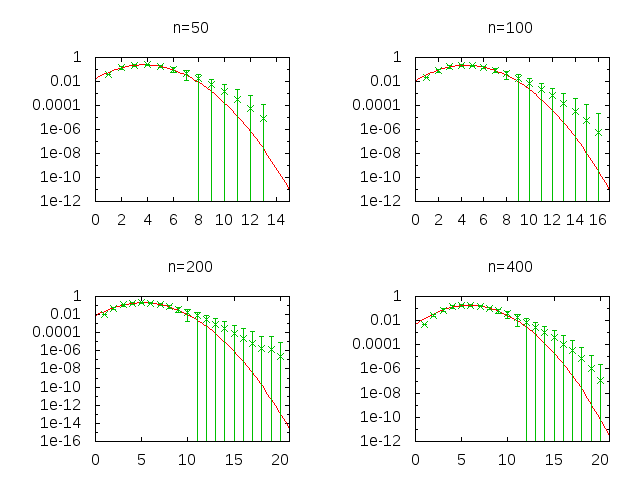
\includegraphics[width=1\linewidth]{../Results/wErrorbars_Normal_M1.png}
  \caption{Fitting an eine Normalverteilung}
\end{subfigure}%
\begin{subfigure}{.5\textwidth}
  \centering
  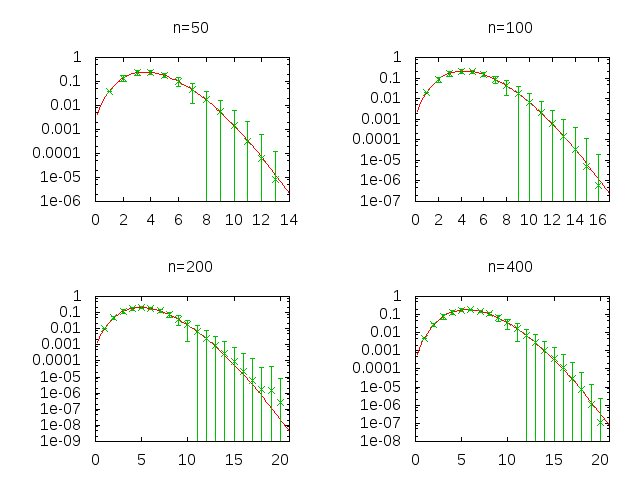
\includegraphics[width=1\linewidth]{../Results/wErrorbars_Power_M1.png}
  \caption{Fitting an Potenzgesetz}
\end{subfigure}
\caption{Skalenfreie Graphen mit $m=1$}
\label{fig:m1}
\end{figure}

Unabhängig von der Anzahl an Knoten scheint der Fit an das Potenzgesetz hier wesentlich besser zu sein. Dies ist im Falle $m=2$ umgekehrt. Hier lässt sich feststellen, dass für ein Fitting an eine Normalverteilung geringere Abweichungen vorliegen. Die Ergebnisse sind in Abbildung \ref{fig:m2} zu sehen.

\begin{figure}[htb!]
\begin{subfigure}{.5\textwidth}
  \centering
  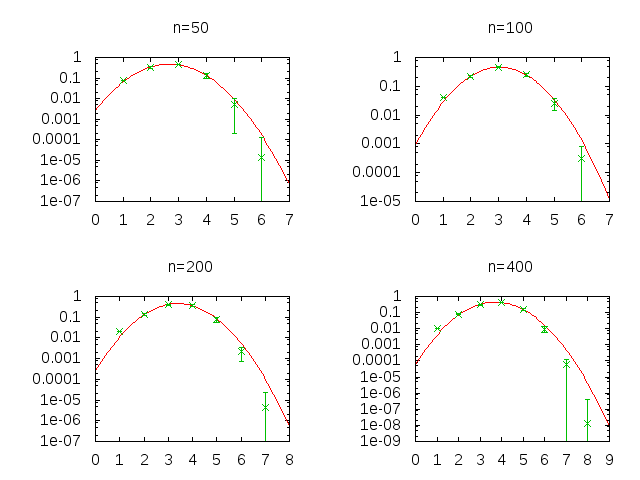
\includegraphics[width=1\linewidth]{../Results/wErrorbars_Normal_M2.png}
  \caption{Fitting an eine Normalverteilung}
\end{subfigure}%
\begin{subfigure}{.5\textwidth}
  \centering
  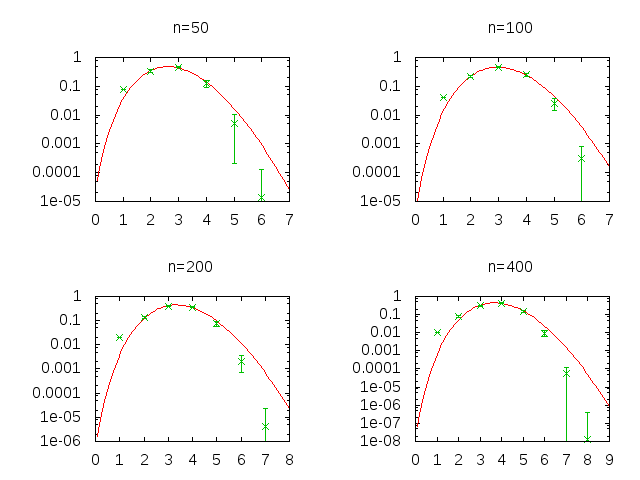
\includegraphics[width=1\linewidth]{../Results/wErrorbars_Power_M2.png}
  \caption{Fitting an Potenzgesetz}
\end{subfigure}
\caption{Skalenfreie Graphen mit $m=2$}
\label{fig:m2}
\end{figure}

Somit lässt sich also schlussfolgern, dass für $m=1$ die Verteilung der kürzesten Wege im Graphen unabhängig von der Größe dem gleichen Gesetz folgt wie es für die Gradverteilung der Knoten gilt, nämlich dem Potenzgesetz. Ändert man den für das preferential attachment massgeblichen Parameter auf $m=2$ so gilt dies nicht mehr, jetzt sind die kürzesten Weglängen im Graphen eher normalverteilt. 

\subsection{Skalenfreie Graphen: Allgemeines preferential attachment}
Für skalenfreie Graphen wurde die Funktion $preferential$ $attachment$ durch einen konstanten Wert $k_0$ erweitert. Dieser beeinflusst die Wahrscheinlichkeit mit der die Knoten miteinander verbunden werden. Durch addition bzw. subtraktion der Konstanten $k_0$ ist die Wahrscheinlichkeit einen existierenden Knoten bei der Graphenerstellung als Nachbarn auszuwählen, also nicht mehr ausschließlich von dessen Grad abhängig. (Aufruf $./simulationConstant.scr$) 

\begin{itemize}
\item[\quad Größe $n$:] $50,100,200,400$
\item[\quad Parameter $m$:] $2$
\item[\quad Konstante $k_0$:] $-1.5,-0.5,0.5,2$
\end{itemize}


\subsection{Ebene Zufallsgraphen}
Für ebene Zufallsgraphen wurden die gleichen Simulationen wie für skalenfreie Graphen durchgeführt (Aufruf: $simulationPlanar.scr$). Der Parameter $m$ spielt hier keine Rolle.
\begin{itemize}
\item[\quad Größe $n$:] $50,100,200,400$
\end{itemize}
Es zeigt sich, dass auch hier eine Normalverteilung die bessere Approximation liefert (siehe Abbildung \ref{fig:planar}).

\begin{figure}[htb!]
\begin{subfigure}{.5\textwidth}
  \centering
  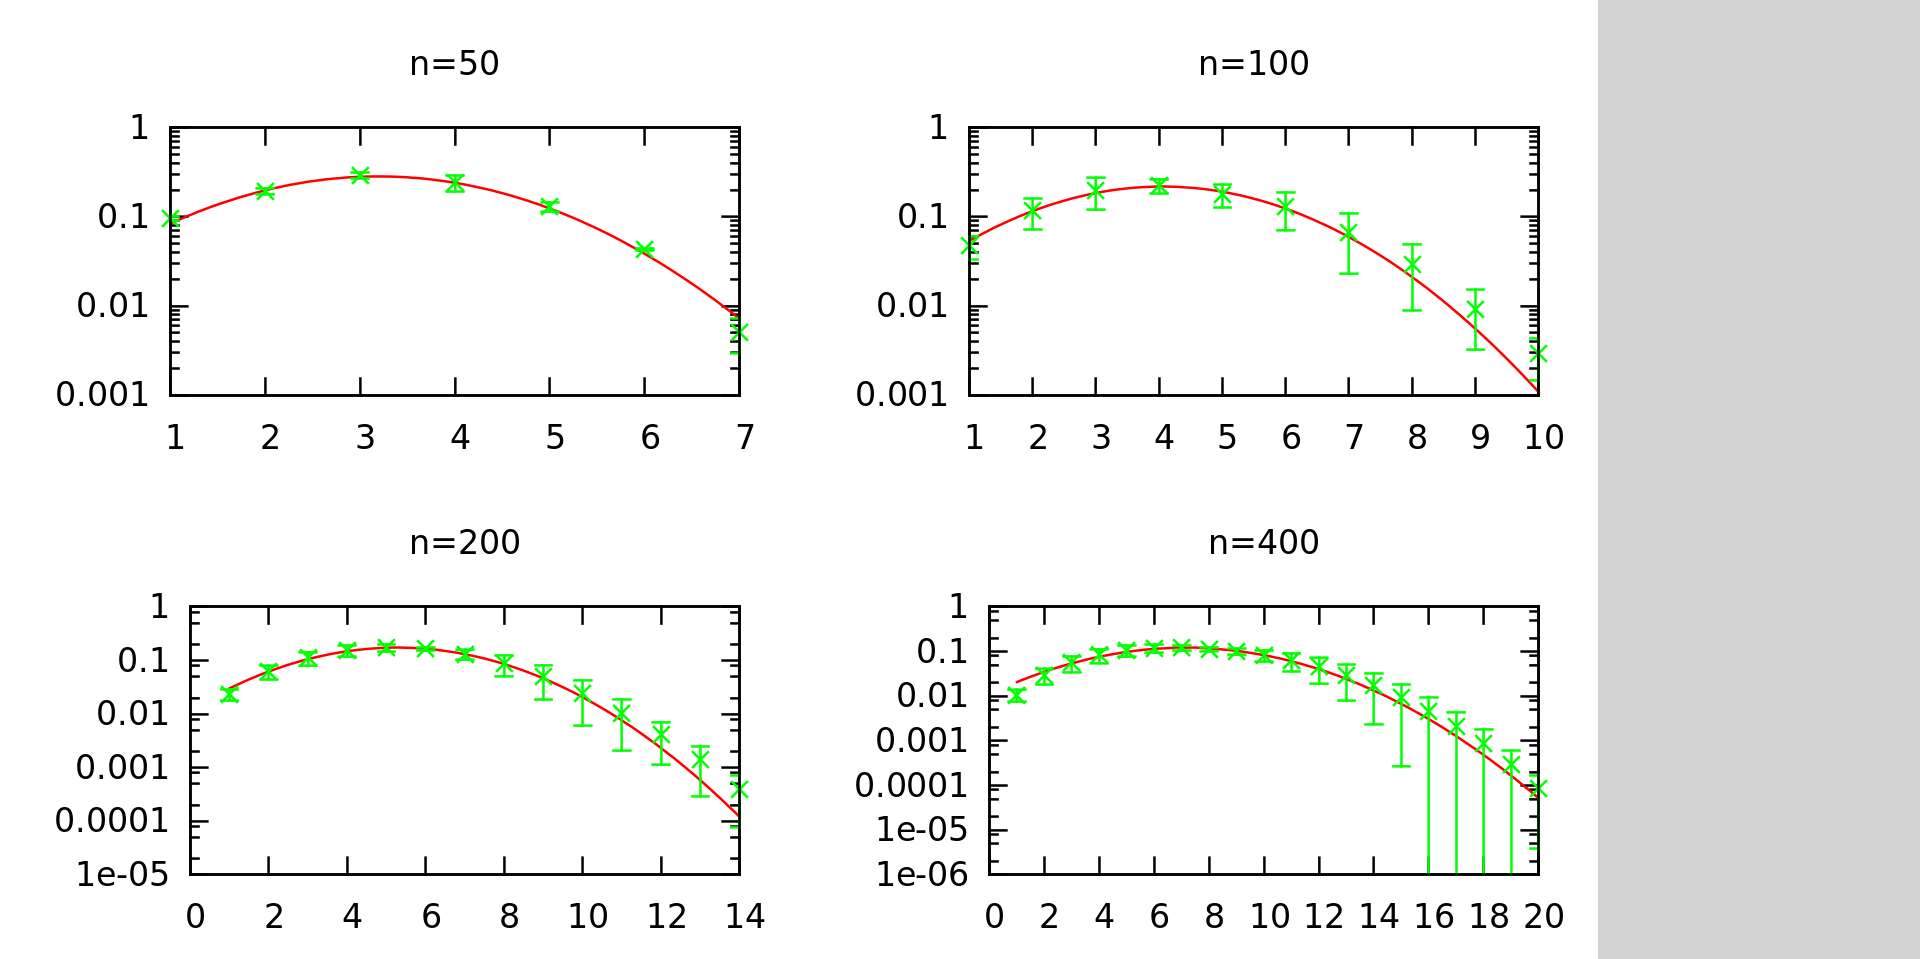
\includegraphics[width=\linewidth]{../Results/wErrorbars_Normal_Planar.png}
  \caption{Fitting an eine Normalverteilung}
\end{subfigure}%
\begin{subfigure}{.5\textwidth}
  \centering
  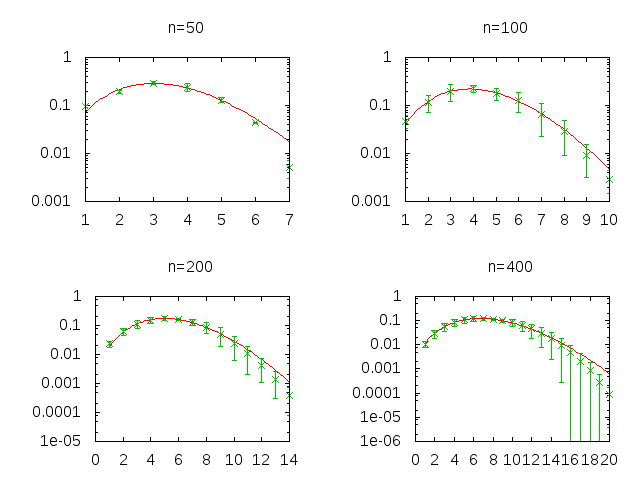
\includegraphics[width=\linewidth]{../Results/wErrorbars_Power_Planar.png}
  \caption{Fitting an Potenzgesetz}
\end{subfigure}
\caption{Ebene Zufallsgraphen}
\label{fig:planar}
\end{figure}

\subsection{Mittlere Weglänge in ebenen Zufallsgraphen}
Für ebene Zufallsgraphen wurde zusätzlich untersucht, wie sich die mittlere kürzeste Wegelänge in Abhängigkeit von der Anzahl der Knoten verhält. Es wurden also hier eine größere Menge an Graphgrößen untersucht:
\begin{itemize}
\item[\quad Größe $n$:] $10..1000$, in 10er Schritten
\end{itemize}
Die mittlere Kürzeste-Weglänge konvergiert offenbar gegen einen Wert und der Fit an Potenzgesetze $N^\beta$ scheint gut zu passen. Wir erhalten hier einen Wert von $B= -0.0741915$ mit einem Fehler von $+/- 0.001517$.
\begin{figure}[!htb]
  \centering
  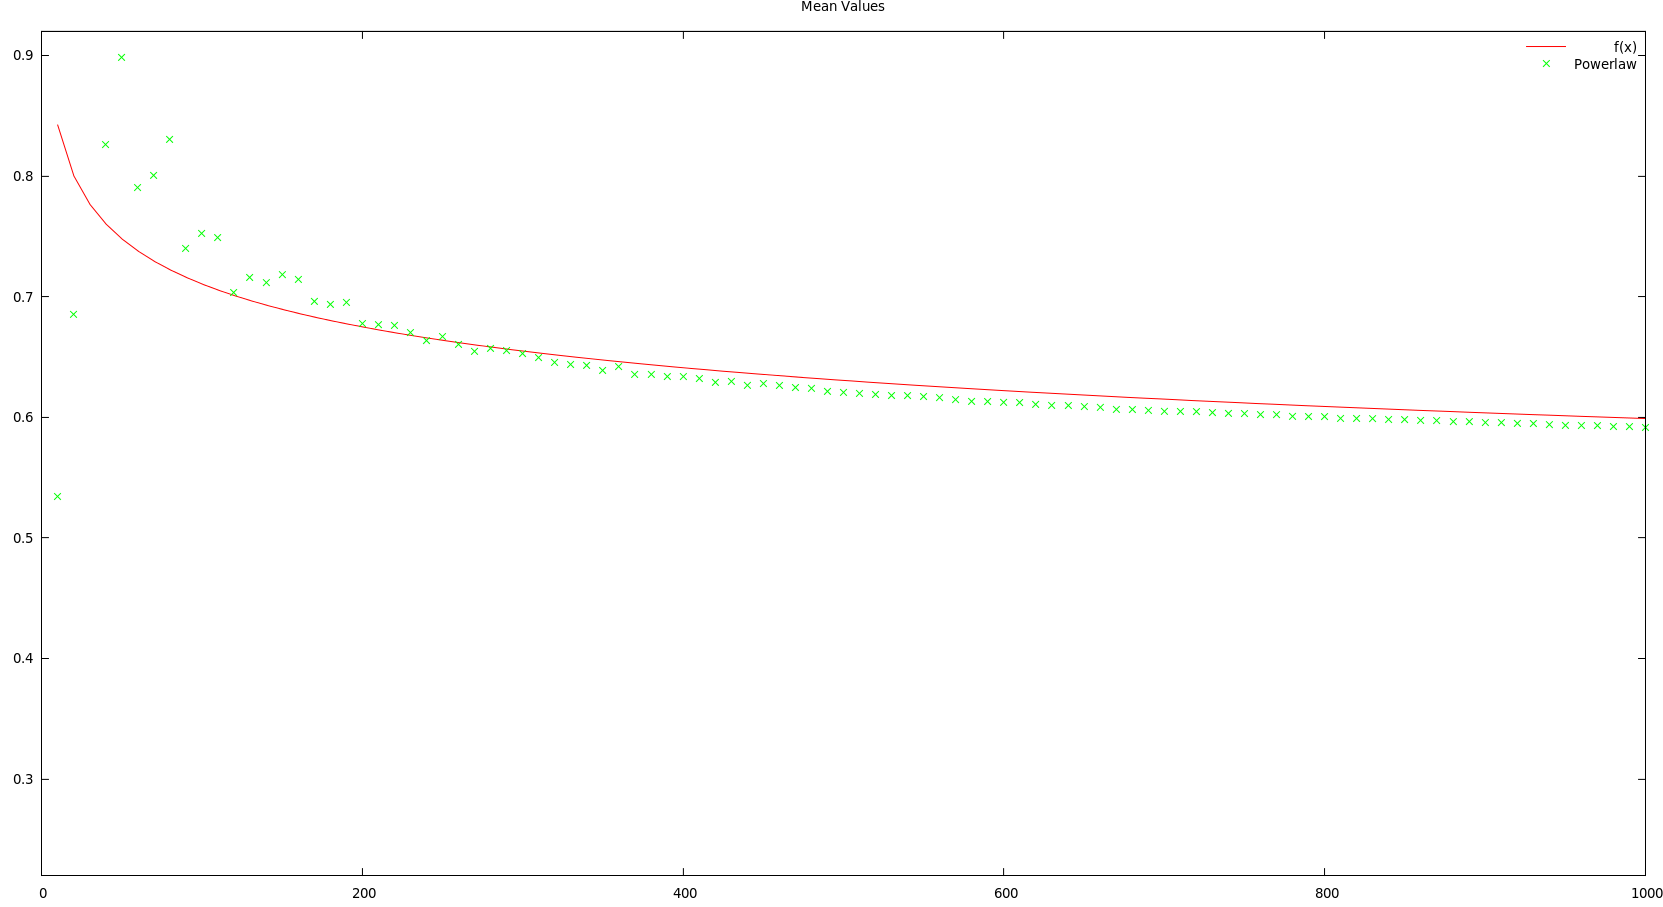
\includegraphics[width=\linewidth]{../Results/Power_PlanarMean.png}
  \caption{Fitting Power Law}
\label{fig:planarMean}
\end{figure}

\section{Fazit}
Lirum Larum Opsum

\newpage

\bibliography{ref} 
\bibliographystyle{ieeetr}

\end{document} 
